%%%%%%%%%%%%%%%%%%%%%%%%%%%%%%%%%%%%%%%%%
% Masters/Doctoral Thesis 
% LaTeX Template
% Version 2.5 (27/8/17)
%
% This template was downloaded from:
% http://www.LaTeXTemplates.com
%
% Version 2.x major modifications by:
% Vel (vel@latextemplates.com)
%
% This template is based on a template by:
% Steve Gunn (http://users.ecs.soton.ac.uk/srg/softwaretools/document/templates/)
% Sunil Patel (http://www.sunilpatel.co.uk/thesis-template/)
%
% Template license:
% CC BY-NC-SA 3.0 (http://creativecommons.org/licenses/by-nc-sa/3.0/)
%
%%%%%%%%%%%%%%%%%%%%%%%%%%%%%%%%%%%%%%%%%

%----------------------------------------------------------------------------------------
%	PACKAGES AND OTHER DOCUMENT CONFIGURATIONS
%----------------------------------------------------------------------------------------

\documentclass[
12pt, % The default document font size, options: 10pt, 11pt, 12pt
%oneside, % Two side (alternating margins) for binding by default, uncomment to switch to one side
italian, % ngerman for German
onehalfspacing, % Single line spacing, alternatives: onehalfspacing or doublespacing
%singlespacing, % Single line spacing, alternatives: onehalfspacing or doublespacing
%draft, % Uncomment to enable draft mode (no pictures, no links, overfull hboxes indicated)
%nolistspacing, % If the document is onehalfspacing or doublespacing, uncomment this to set spacing in lists to single
%liststotoc, % Uncomment to add the list of figures/tables/etc to the table of contents
%toctotoc, % Uncomment to add the main table of contents to the table of contents
%parskip, % Uncomment to add space between paragraphs
%nohyperref, % Uncomment to not load the hyperref package
headsepline, % Uncomment to get a line under the header
%chapterinoneline, % Uncomment to place the chapter title next to the number on one line
%consistentlayout, % Uncomment to change the layout of the declaration, abstract and acknowledgements pages to match the default layout
]{MastersDoctoralThesis} % The class file specifying the document structure

\usepackage[utf8]{inputenc} % Required for inputting international characters
\usepackage[T1]{fontenc} % Output font encoding for international characters
\usepackage{listings}

\lstset{ 
  basicstyle=\footnotesize\ttfamily,
  % numbers=left,
  showspaces=false,
  columns=fullflexible
}

\lstdefinestyle{customc}{
  basicstyle=\footnotesize\ttfamily,
  numbers=left,
  showspaces=false,
  columns=fullflexible,
  captionpos=b
}

\renewcommand{\lstlistingname}{Codice}

\usepackage{mathpazo} % Use the Palatino font by default
\usepackage{tabularx}
\usepackage{marginnote}

\usepackage[backend=bibtex,style=authoryear,natbib=true]{biblatex} % Use the bibtex backend with the authoryear citation style (which resembles APA)

\addbibresource{example.bib} % The filename of the bibliography

\usepackage[autostyle=true]{csquotes} % Required to generate language-dependent quotes in the bibliography

%----------------------------------------------------------------------------------------
%	MARGIN SETTINGS
%----------------------------------------------------------------------------------------

\geometry{
	paper=a4paper, % Change to letterpaper for US letter
	inner=2.5cm, % Inner margin
	outer=3.8cm, % Outer margin
	bindingoffset=.5cm, % Binding offset
	top=1.5cm, % Top margin
	bottom=1.5cm, % Bottom margin
	%showframe, % Uncomment to show how the type block is set on the page
}

%----------------------------------------------------------------------------------------
%	THESIS INFORMATION
%----------------------------------------------------------------------------------------

\thesistitle{Migrazione da iptable a nftables} % Your thesis title, this is used in the title and abstract, print it elsewhere with \ttitle
\supervisor{Dottr. James \textsc{Smith}} % Your supervisor's name, this is used in the title page, print it elsewhere with \supname
\examiner{} % Your examiner's name, this is not currently used anywhere in the template, print it elsewhere with \examname
\degree{Doctor of Philosophy} % Your degree name, this is used in the title page and abstract, print it elsewhere with \degreename
\author{Marco \textsc{De Benedetto}} % Your name, this is used in the title page and abstract, print it elsewhere with \authorname
\addresses{} % Your address, this is not currently used anywhere in the template, print it elsewhere with \addressname

\subject{Linux firewall} % Your subject area, this is not currently used anywhere in the template, print it elsewhere with \subjectname
\keywords{} % Keywords for your thesis, this is not currently used anywhere in the template, print it elsewhere with \keywordnames
\university{\href{http://www.university.com}{University Name}} % Your university's name and URL, this is used in the title page and abstract, print it elsewhere with \univname
\department{\href{http://department.university.com}{Department or School Name}} % Your department's name and URL, this is used in the title page and abstract, print it elsewhere with \deptname
\group{\href{http://researchgroup.university.com}{Research Group Name}} % Your research group's name and URL, this is used in the title page, print it elsewhere with \groupname
\faculty{\href{http://faculty.university.com}{Faculty Name}} % Your faculty's name and URL, this is used in the title page and abstract, print it elsewhere with \facname

\AtBeginDocument{
\hypersetup{pdftitle=\ttitle} % Set the PDF's title to your title
\hypersetup{pdfauthor=\authorname} % Set the PDF's author to your name
\hypersetup{pdfkeywords=\keywordnames} % Set the PDF's keywords to your keywords
}

\begin{document}

\frontmatter % Use roman page numbering style (i, ii, iii, iv...) for the pre-content pages

\pagestyle{plain} % Default to the plain heading style until the thesis style is called for the body content

%----------------------------------------------------------------------------------------
%	TITLE PAGE
%----------------------------------------------------------------------------------------

\begin{titlepage}
\begin{center}

\vspace*{.06\textheight}
{\scshape\LARGE \univname\par}\vspace{1.5cm} % University name
\textsc{\Large Project Work Master Cybersecurity}\\[0.5cm] % Thesis type

\HRule \\[0.4cm] % Horizontal line
{\huge \bfseries \ttitle\par}\vspace{0.4cm} % Thesis title
\HRule \\[1.5cm] % Horizontal line
 
\begin{minipage}[t]{0.4\textwidth}
\begin{flushleft} \large
\emph{Autore:}\\
\href{https://github.com/marcodebe}{\authorname} % Author name - remove the \href bracket to remove the link
\end{flushleft}
\end{minipage}
\begin{minipage}[t]{0.4\textwidth}
\begin{flushright} \large
\emph{Tutor:} \\
\supname % Supervisor name - remove the \href bracket to remove the link  
\end{flushright}
\end{minipage}\\[3cm]
 
\vfill

\large \textit{A thesis submitted in fulfillment of the requirements\\ for the degree of \degreename}\\[0.3cm] % University requirement text
\textit{in the}\\[0.4cm]
\groupname\\\deptname\\[2cm] % Research group name and department name
 
\vfill

{\large \today}\\[4cm] % Date
%\includegraphics{Logo} % University/department logo - uncomment to place it
 
\vfill
\end{center}
\end{titlepage}

%----------------------------------------------------------------------------------------
%	DECLARATION PAGE
%----------------------------------------------------------------------------------------

% \begin{declaration}
% \addchaptertocentry{\authorshipname} % Add the declaration to the table of contents
% \noindent I, \authorname, declare that this thesis titled, \enquote{\ttitle} and the work presented in it are my own. I confirm that:
% 
% \begin{itemize} 
% \item This work was done wholly or mainly while in candidature for a research degree at this University.
% \item Where any part of this thesis has previously been submitted for a degree or any other qualification at this University or any other institution, this has been clearly stated.
% \item Where I have consulted the published work of others, this is always clearly attributed.
% \item Where I have quoted from the work of others, the source is always given. With the exception of such quotations, this thesis is entirely my own work.
% \item I have acknowledged all main sources of help.
% \item Where the thesis is based on work done by myself jointly with others, I have made clear exactly what was done by others and what I have contributed myself.\\
% \end{itemize}
%  
% \noindent Signed:\\
% \rule[0.5em]{25em}{0.5pt} % This prints a line for the signature
%  
% \noindent Date:\\
% \rule[0.5em]{25em}{0.5pt} % This prints a line to write the date
% \end{declaration}
% 
% \cleardoublepage
% 
% %----------------------------------------------------------------------------------------
% %	QUOTATION PAGE
% %----------------------------------------------------------------------------------------
% 
% \vspace*{0.2\textheight}
% 
% \noindent\enquote{\itshape Thanks to my solid academic training, today I can write hundreds of words on virtually any topic without possessing a shred of information, which is how I got a good job in journalism.}\bigbreak
% 
% \hfill Dave Barry
% 
% %----------------------------------------------------------------------------------------
% %	ABSTRACT PAGE
% %----------------------------------------------------------------------------------------
% 
\begin{abstract}
\addchaptertocentry{\abstractname} % Add the abstract to the table of contents
Studio ed realizzazione di migrazioi di firewall Linux da iptables a nftables.

\end{abstract}


%----------------------------------------------------------------------------------------
%	ACKNOWLEDGEMENTS
%----------------------------------------------------------------------------------------
%
%\begin{acknowledgements}
%\addchaptertocentry{\acknowledgementname} % Add the acknowledgements to the table of contents
%The acknowledgments and the people to thank go here, don't forget to include your project advisor\ldots
%\end{acknowledgements}
%
%----------------------------------------------------------------------------------------
%	LIST OF CONTENTS/FIGURES/TABLES PAGES
%----------------------------------------------------------------------------------------

\tableofcontents % Prints the main table of contents

\listoffigures % Prints the list of figures

\listoftables % Prints the list of tables

%----------------------------------------------------------------------------------------
%	ABBREVIATIONS
%----------------------------------------------------------------------------------------

%\begin{abbreviations}{ll} % Include a list of abbreviations (a table of two columns)

%\textbf{NAT} & \textbf{N}etwork \textbf{A}ddress \textbf{T}ranslation\\
%\textbf{SNAT} & \textbf{S}ource \textbf{N}etwork \textbf{A}ddress \textbf{T}ranslation\\
%\textbf{DNAT} & \textbf{D}estination \textbf{N}etwork \textbf{A}ddress \textbf{T}ranslation\\
%\textbf{WSF} & \textbf{W}hat (it) \textbf{S}tands \textbf{F}or\\
%
%\end{abbreviations}

%----------------------------------------------------------------------------------------
%	PHYSICAL CONSTANTS/OTHER DEFINITIONS
%----------------------------------------------------------------------------------------

%\begin{constants}{lr@{${}={}$}l} % The list of physical constants is a three column table
%
%% The \SI{}{} command is provided by the siunitx package, see its documentation for instructions on how to use it
%
%Speed of Light & $c_{0}$ & \SI{2.99792458e8}{\meter\per\second} (exact)\\
%%Constant Name & $Symbol$ & $Constant Value$ with units\\
%
%\end{constants}

%----------------------------------------------------------------------------------------
%	SYMBOLS
%----------------------------------------------------------------------------------------

%\begin{symbols}{lll} % Include a list of Symbols (a three column table)
%
%$a$ & distance & \si{\meter} \\
%$P$ & power & \si{\watt} (\si{\joule\per\second}) \\
%%Symbol & Name & Unit \\
%
%\addlinespace % Gap to separate the Roman symbols from the Greek
%
%$\omega$ & angular frequency & \si{\radian} \\
%
%\end{symbols}

%----------------------------------------------------------------------------------------
%	DEDICATION
%----------------------------------------------------------------------------------------

%\dedicatory{For/Dedicated to/To my\ldots} 

%----------------------------------------------------------------------------------------
%	THESIS CONTENT - CHAPTERS
%----------------------------------------------------------------------------------------

\mainmatter % Begin numeric (1,2,3...) page numbering

\pagestyle{thesis} % Return the page headers back to the "thesis" style

% Include the chapters of the thesis as separate files from the Chapters folder
% Uncomment the lines as you write the chapters

%\include{Chapters/Chapter1}
%\include{Chapters/Chapter2} 
%\include{Chapters/Chapter3}
%\include{Chapters/Chapter4} 
%\include{Chapters/Chapter5} 

%Indice

%Premessa
%Cenni storici
%Descrizione Firewall Galliera
%Migrazione FW interno
%  Simulazione con lxc
%  Sistemi di automazione
%Il futuro
%  {\em iptables}
%  eBPF/XDP

\chapter{Introduzione} % Main chapter title

\label{Chapter1} % For referencing the chapter elsewhere, use \ref{Chapter1} 

%----------------------------------------------------------------------------------------

% Define some commands to keep the formatting separated from the content 
\newcommand{\keyword}[1]{\textbf{#1}}
\newcommand{\tabhead}[1]{\textbf{#1}}
\newcommand{\code}[1]{\texttt{#1}}
\newcommand{\file}[1]{\texttt{\bfseries#1}}
\newcommand{\option}[1]{\texttt{\itshape#1}}

%----------------------------------------------------------------------------------------

Il progetto di seguito presentato ha avuto origine da considerazioni
relative alla necessit\`a di aggiornare il sistema di firewall a protezione
della rete interna dell'ospedale Galliera.

La LAN dell'ospedale \`e connessa ad internet dal 1996 e sin da allora il
traffico di rete da e verso l'esterno \`e stato regolato e monitorato da
router/firewall Linux da me opportunamente configurati.

Nel tempo le esigenze di connettivit\`a sono via via aumentate ed i nostri
sistemi si sono dimostrati adeguati sia per quanto riguarda le funzionalit\`a
che per prestazioni.

Tuttavia nell'arco del 2017 si sono presentate alcune situazioni di
criticit\`a, causate sostanzialmente dal grande numero di regole sul firewall.

Pur essendo riuscito a risolvere i problemi ho ritenuto di dover considerare
questi segnali di possibile obsolescenza del sistema, studiando le attuali
alternative agli strumenti scelti oramai circa 17 anni fa: cio\`e in pratica
le alternative ad iptables.  In effetti l'alternativa c'\`e: si chiama
nftables ed il suo scopo è proprio quello di soppiantare iptables
superandone tutte le limitazioni.

Il progetto di migrazione da iptables a nftables \`e consistito prima di
tutto nello studio del nuovo sistema, nella riorganizzazione delle regole dei
due firewall (operazione ancora in corso), e nella preparazione di scenari di
test usando macchine virtuali.

%\chapter{}
%Nel frattempo l'analisi dello stato delle cose del kernel Linux ha evidenziato
%una recente presa di posizione di molti, tra cui importanti sviluppatori e
%aziende, che sostiene l'impossibilit\`a di elim
%
%Netfilter è un framework implementato da Linux che permette di
%compiere diverse operazioni relative al traffico di rete: packet-filtering,
%nat, mangling, etc.
%
%I predecessori di iftables sono stati {\em ipfwadm} per i kernel dall'1.2.x (con x>0)
%al 2.0.x (1995-1999), {\em ipchains} per i kernel 2.2.x (1999-2001).  {\em iptables} è
%presente dal kernel 2.4.x in poi (2001).
%
%L'attuale (2018) kernel è il 4.15.9 e tuttora, su Linux, {\em iptables} è lo
%strumento di packet-filtering più utilizzato sia come firewall limitato al
%singolo host, sia per la protezione di sotto-reti e per la realizzazione di
%diverse soluzioni che richiedano analisi, classificazione, elaborazione e
%modifica di pacchetti di rete in transito.
%
%{\em iptables} è quindi in produzione da cira 17 anni anche se, a partire dalla
%versione di kernel 3.13 (gennaio 2014
%https://kernelnewbies.org/Linux\_3.13\#nftables.2C\_the\_successor\_of\_{\em iptables}),
%Linux offre uno nuovo strumento alternativo ad {\em iptables}: nftables. Nftables
%appare per la prima volta nel 2009 (https://lwn.net/Articles/564095/) ma il
%progetto langue fino al 2014 quando torna ad attirare l'attenzione degli
%sviluppatori interessati a sopperire ai difetti di progettazione e alle carenze
%di {\em iptables}.
%
%{\em iptables} è composto in realtà da un insieme di componenti separate e ognuna di
%esse ha consapevolezza del singolo protocollo che gestisce ― ipv4, ipv6,
%Ethernet bridging, ARP - il codice è quindi replicato quattro volte.
%
%Questa situazione è frustrante per gli sviluppatori e l'idea di un nuovo
%sistema di packet filtering unico e /general purpose/ rende accettabile lo
%sforzo necessario all'introduzione di un'ulteriore macchina virtuale (VM) nel
%kernel.
%
%L'idea di una VM che esegua bytecode nel kernel potrebbe sembrare, dal punto di
%vista delle prestazioni, un errore; tuttavia ci si rende invece conto che il
%bytecode può offrire prestazioni migliori del codice che sostituisce.  Inoltre
%nftables introduce sostanziali miglioramenti rispetto al predecessore.
%
%Quel che succede però è che nftables non rimpiazza {\em iptables}: lo affianca.  A
%differenza dei suoi predecessori non esiste quindi una versione di kernel a
%partire dalla quale il vecchio sistema non è più supportato.
%
%Uno dei motivi, a mio parere uno dei principali, per cui nftables non ha
%soppiantato da un giorno all'altro {\em iptables} consiste nella vasta adozione di
%{\em iptables} a tutti i livelli, dai singoli host, ai dispositivi (cosiddetti IoT) e
%soprattutto nei grandi datacenter (cloud).

\chapter{Packet Filtering in Linux}

\label{Cenni storici} % For referencing the chapter elsewhere, use \ref{Chapter1} 

Per inquadrare l'argomento Linux firewall ritengo possa essere interessante
fornire un breve riassunto dell'evoluzione degli strumenti per la
classificazione ed il filtraggio dei pacchetti nel kernel Linux.

\section{Storia}
Nella tabella \ref{tab:history}
vengono considerate solo i rilasci nei kernel stabili. Fino alla serie 2.6.x le
nuove fetures venivano introdotte sperimentalmente nelle versioni con major
revision number dispari, ad esempio 2.3.4; dalla versione 3 questo cambia e non
esiste più la differenza tra kernel sperimentale e di produzione.
\begin{center}
  \label{tab:history}
  \begin{table}[ht]
    \centering % used for centering table
     \begin{tabular}{@{}lcccl@{}}
       \toprule
       {\bf Framework/tool} & {\bf Stateful} & {\bf Anno} & {\bf Kernel} & {\bf Coder}\\ \midrule
       ipfw     & no & 1994      & 1.0  & Alan Cox \\
       ipfwadm  & no & 1995-1999 & 1.2.$x$\marginnote{con $x>0$} - 2.0 & A. Cox e Jos Vos\\ [0.5ex]
       ipchains & no & 1999-2001 & 2.2  & Rusty Russell \\ [0.5ex]
       iptables & s\`i & 2001-     & 2.4  & Rusty Russell \\ [0.5ex]
       nftables & s\`i & 2014-     & 3.13 & gli stessi di iptables \\ [0.5ex]
       %eBPF/XDP & s\`i &       &      & \\ 
       \bottomrule
     \end{tabular}  
    \caption{Evoluzione dei tool (kernel versioni stabili)} % title of Table
  \end{table}
\end{center}
Le prime funzionalità di firewall sono state introdotte nel 1994 grazie al
lavoro di Alan Cox che ne ha fatto il porting da BSD.
Questo codice costituisce la prima versione delle funzionalità di firewall
all'interno del kernel Linux. Il successore di ipfw è
stato ipfwadm, in realtà una riscrittura del corrispondente ipfw
di BSD da parte di Alan Cox e Jos Vos.
Ipfw e ipfwadm consentivano di realizzare funzioni di base di un firewall:
\begin{itemize}
    \item accounting di pacchetti IP,
    \item firewall di ingresso,
    \item firewall di uscita,
    \item firewall di inoltro,
    \item redirezione (permette proxy trasparente)
    \item masquerading
\end{itemize}
A partire dal kernel Linux 2.2 (1999) viene rilasciato un nuovo sistema di packet
filtering: ipchains. Ipchains \`e sostanzialmente una completa
riscrittura del codice di ipfw di cui espande le funzionalità.  In particolare
ipchains gestisce ulteriori protocolli oltre a TCP, UDP e ICMP, ed inoltre è
in grado di gestire la frammentazione dei pacchetti.

Anche ipchains come ipfwadm realizza però un firewall non stateful; l'unica
opzione che ha per decidere se accettare un pacchetto entrante consiste nel
verificare se il bit ACK \`e settato (significa che si tratta di una risposta
relativa ad una connessione già stabilita), ma questo significa fidarsi del
pacchetto di cui si deve stabilire il verdetto.  Ovviamente questa politica è
inerentemente poco sicura in quanto è facile inviare pacchetti costruiti ad
arte per superare i filtri del firewall.

Nel kernel 2.4 assistiamo nuovamente ad una completa riscrittura delle
funzionalità di filtro e firewall di Linux, viene introdotto il framework 
Netfilter (comunemente noto come iptables).

\section{Netfilter}
Netfilter è molto più maturo rispetto ai suoi predecessori, permette di
realizzare firewall stateful con maggiori capacità di ispezione dei pacchetti
e capacità di log.

Alcune delle caratteristiche di Netfilter sono:

\begin{itemize}
    \item Stateless packet filtering per IPv4 e IPV6
    \item Stateful packet filtering per IPv4 (inizialmente, in seguito
        aggiunto il supporto per IPv6 (2.6.15)
    \item Network e Port address translation (NAT e NAPT)
    \item Infrastruttura flessibile ed estendibile
    \item API per estensioni di terze parti
    \item Un gran numero di plugin/moduli
\end{itemize}
Per queste caratteristiche, ed essendo software libero che riceve
grande supporto della comunità open source, i firewall basati su Linux
iniziarono ad essere sviluppati anche in forma di prodotti commerciali offerti
da diverse aziende che ne forniscono supporto tecnico.

Il tool di configurazione di Netfilter, che è poi il nome col quale è noto il
framework stesso, è iptables.
In realtà gli strumenti di configurazione del framework Netfilter formano una
famiglia: oltre a iptables, che gestisce regole IPv4, esistono ip6tables per
regole IPV6, ebtables per realizzare firewall layer 2 (Linux Bridge)
e arptables che lavora nello specifico su messaggi ARP.

Ai diversi tool corrispondono, nel kernel, porzioni di codice ad-hoc per il
singolo protocollo: IPv4, IPv6, EB (Ethernet Bridge), ARP.  A volte si usa
il termine Xtables per definire l'intera famiglia.

La possibilità di aggiungere plugin ha fatto s\'i che nel tempo Xtables si
sia arricchito di molti moduli aggiuntivi.

A partire dal kernel 3.13 (2014) viene introdotto nftables con l'intento
di soppiantare iptables.  Il nuovo framework di classificazione di pacchetti
nasce con lo scopo di superare quelli che vengono considerati difetti o
carenze di iptables.
\begin{figure}[H]
    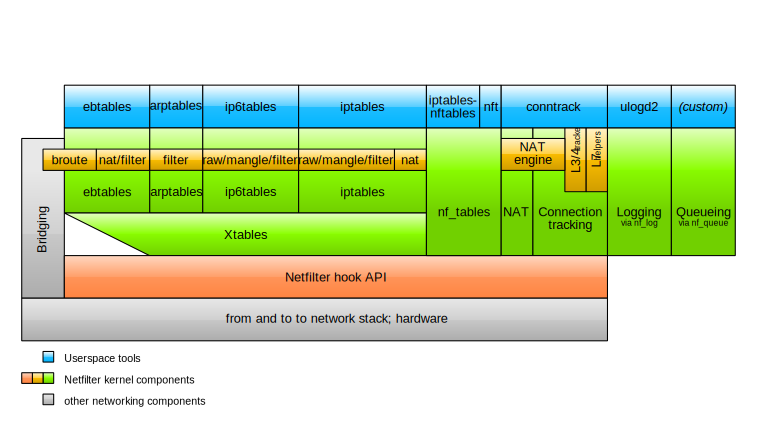
\includegraphics[width=\linewidth]{nf-components.eps}
    \caption[Componenti di Netfilter]{Componenti di Netfilter:\footnotemark}
    \label{fig:netfilter}
\end{figure}
\noindent Dalla figura \ref{fig:netfilter} risulta evidente la maggiore complessità e
\footnotetext{\href{http://inai.de/images/nf-components.svg}{Sorgente} (CC BY-SA 3.0).}%
ridondanza di Xtables rispetto a nftables.  Nftables riduce il numero di linee
di codice nel kernel riorganizzando e unificando quello che in iptables è
replicato per i diversi protocolli.  Inoltre nftables introduce strutture
dati, insiemi\footnote{Iptables non gestisce nativamente gli insiemi ma esiste
il tool ipset che fornisce a iptables questa funzionalità.}, dizionari e mappe,
che permettono di semplificare e ottimizzare le regole del firewall.
Migliorano anche la leggibilità delle regole e le prestazioni.

Un'altra caratteristica molto importante consiste nel fatto che con iptables
ogni regola viene introdotta dal comando iptables con relativi
argomenti; nftables invece consiste di un vero e proprio linguaggio nel quale
viene descritto e configurato l'intero firewall; inoltre le regole vengono
attivate atomicamente.

\chapter{Firewall Linux nella rete Galliera}
\section{Cenni storici}

La LAN dell'ospedale Galliera è collegata ad internet dal 1996 e sin
dall'inizio ho utilizzato macchine Linux per i servizi di rete e per
realizzare firewall.  La prima versione, del 1996, di router/firewall l'ho
realizzata con ipfwadm.

Ad ogni evoluzione dei sistemi di firewall di Linux ho provveduto ad
aggiornare i sistemi convertendo di volta in volta le regole e approffittando
delle nuove funzionalità introdotte.  Nei casi precedenti ad nftables, la
migrazione si rendeva necessaria anche perché il vecchio framework veniva
dichiarato obsoleto e non più supportato.  Questo non è ancora accaduto per
iptables e tutto fa pensare che in questo caso il percorso sarà diverso;
vedremo in seguito i dettagli di come si possa prospettare la transizione da
iptables al suo successore (che come vedremo potrebbe non essere nftables).

L'uso del firewall nei primi anni era limitato all'implementazione di filtri
per il traffico in ingresso verso i servizi esposti a internet e al {\em
masquerading} o SNAT (Source Network Address Translation) degli indirizzi IPv4
interni (di classe riservata) per l'inoltro del traffico verso internet.

\section{Architettura attuale}
Nel tempo è cresciuto il numero di sottoreti collegate, di servizi esposti e
di conseguenza la complessità delle regole configurate.

La situazione attuale consiste di due firewall Linux, uno esterno ed uno
interno.  Il firewall esterno regola il traffico tra internet, DMZ e reti
locali; quello interno regole il traffico tra le reti locali e l'esterno.

\begin{figure}
\begin{center}
    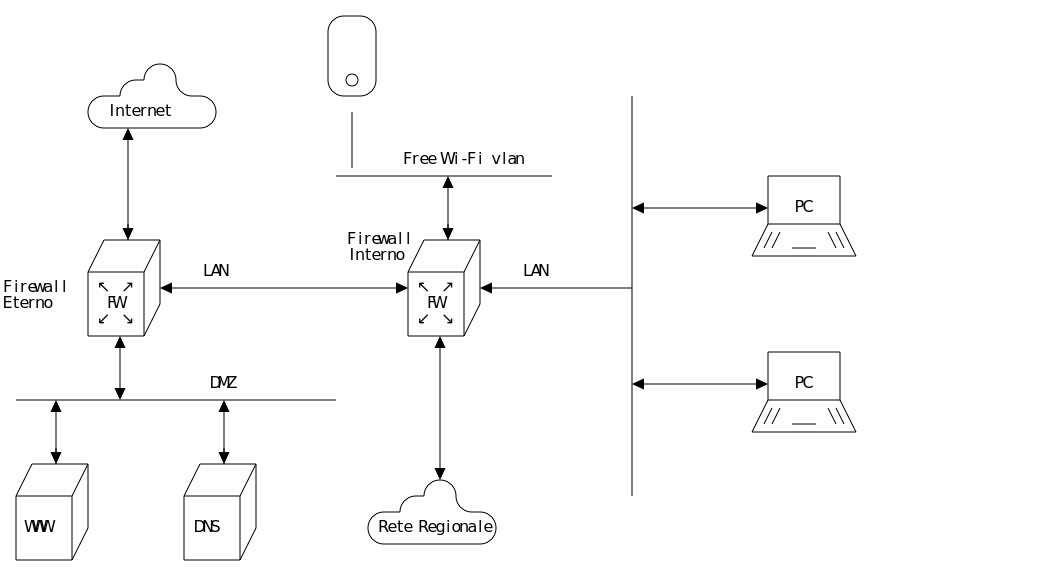
\includegraphics[width=\linewidth]{net.eps}
    \caption{Schema (semplificato) delle reti e dei due firewall}
    \label{fig:rete}
\end{center}
\end{figure}
In particolare sul firewall esterno sono presenti regole di tipo blacklist per
diversi insiemi di indirizzi. Le regole sono aggiorrnate
ogni 5 minuti.  Le liste di indirizzi provengono da:

\begin{itemize}
    \item \href{https://iplists.firehol.org/?ipset=firehol\_level1}{''FireHol
    Level1''}\footnote{https://iplists.firehol.org/?ipset=firehol\_level1} (oltre
    7000 sottoreti),
    \item \href{https://ransomwaretracker.abuse.ch/downloads/RW\_IPBL.txt}{''Ransomware
    Tracker''}\footnote{https://ransomwaretracker.abuse.ch/downloads/RW\_IPBL.txt}
    (circa 400 indirizzi)
    \item fail2ban su ssh: blacklist auto-generata in base ai tentativi
    falliti di connessione via ssh (circa 9000 indirizzi al momemnto)
    \item lista di indirizzi di botnet autoprodotta da script che analizzano
    tentativi di bruteforce tipicamente su servizi di posta (oltre 12.000
    indirizzi)
\end{itemize}
Il totale delle regole supera le 20 mila.

Il firewall interno ha la particolarità di dover gestire le regole del 
Captive Portal: si tratta di abilitare il traffico verso internet dei
dispositivi wireless di coloro che si sono registrati tramite via interfaccia
web.

Il sistema di registrazione e abilitazione, realizzato da me con la
collaborazione di un collega, agisce classificando i pacchetti in base al mac
address: i pacchetti con mac adddress abilitato vengono inoltrati
regolarmente, i rimanenti vengono marcati\footnote{L'associazione del valore
al pacchetto è realizzata all'interno del kernel, il pacchetto resta
inalterato.} e, successivamente, una regola nella catena di inoltro devia il
pacchetto verso il sito del Captive Portal che propone la registrazione.

Abbiamo quasi 100 nuove registrazioni al giorno e sono 100.000 i dispositivi
che hanno usufruito del servizio a partire dal 2012.  Non avendo specificato
termini di scadenza la lista di mac address non decresce mai; ad esempio al
momento sono presenti oltre 23 mila indirizzi ethernet.  Di tanto in tanto si
eseguono interventi di cancellazione delle autorizzazioni pi\`u vecchie.

\section{Problemi dell'infrastruttura}

Nella sezione precedente ho messo in evidenza le dimensioni degli insiemi di
indirizzi e le perché proprio la gestione di così tante regole ha, durante il
2017, portato alla luce alcune carenze della soluzione implementata.

Inizialmente per ogni indirizzo era prevista una regola\footnote{Di tipo {\em
REJECT} per le blacklist e di tipo {\em RETURN} per la gestione della rete wifi
free.}, ciò significa che prima di poter classificare ogni singolo pacchetto
\`e necessario scorrere una per una migliaia, se non decine di migliaia, di
regole (ovviamente non subiscono questa verifica i pacchetti relativi a
connessioni gi\`a stabilite).  Questo approccio non risulta essere efficiente,
superata una certa soglia\footnote{Nella attuale configurazione hardware
questo limite \`e di circa 15 mila regole.}
risultava evidente il carico del server tanto da rendere difficoltoso anche
l'accesso via ssh e l'esecuzione di comandi.

Come accennato in precedenza iptables non prevede strutture dati quali gli
insiemi; esiste per\`o uno strumento esterno, ipset, che fornisce questa
funzionalità permettendo di ridurre decine di migliaia di regole ad un unica
regola (nello specifico una regola per ogni insieme).

I problemi dovuti all'eccessivo numero di regole li ho quindi risolti usando
ipset su entrambe i firewall.  Nel caso del firewall interno è stato anche
necessario aggiornare il kernel ad una versione in grado di gestire insiemi
contenenti mac address.

L'introduzione di ipset ha richiesto, oltre alla modifica della configurazione
dei due firewall, anche le revisione del codice del captive portal e dei
programmi di generazione di black list.

\section{Opportunità di migrazione a nftables}

L'uso di ipset ha risolto i problemi, tuttavia ho voluto verificare cosa
comporti la migrazione da iptables a nftables, in termini di impegno necessario
rispetto ai vantaggi offerti.

Come accennato in precedenza, nftables si propone come framework completamente
nuovo, più che come evoluzione di iptables  e l'interfaccia di configurazione
è diventata un vero e proprio linguaggio di programmazione, a differenza di
iptables dove ogni regola viene inserita da un commando con relativi
argomenti.  Ci\`o significa dover riprogrammare tutte le logiche all'interno
del nuovo framwork.

\chapter{Nftables}

\section{Caratteristiche di nftables}
Vediamo quali sono le principali novit\`a introdotte da nftables.
\begin{itemize}
    \item supporto nativo per dual stack IPv4 e IPv6
    \item supporto nativo per strutture dati (importanti per le prestazioni):
    insiemi, mappe, dizionari e concatenazioni
    \item strumenti di debug e report decisamente migliori
    \item aggiunta dell'hook ingress per migliorare le prestazioni
    \item layout di regole flessibile, partendo da un insieme vuoto, rispetto
    al classico layout statico di iptables (filter/INPUT, nat/PREROUTING,
    \ldots)
    \item contatori opzionali e azioni multiple in una singola regola (ad
    esempio si pu\`o incrementare un contatore, loggare e eseguire NAT nella
    stessa regola)
    \item migliori opzioni di gestione dell'insieme di regole, aggiornamenti
    delle regole completamente atomici e incrementali
\end{itemize}
Si possono quindi inserire regole che valgono contestualemnte sia per IPv4 che
per IPv6,
mentre le strutture dati consentono di migliorare le prestazioni e la
leggibilit\`a delle regole, oltre a non richiedere il supporto di tool
esterni.

Gli strumenti di debug e log sono molto raffinati e utili: \`e ad
esempio possibile tracciare l'intero percorso di un singolo pacchetto
attraverso le regole.  Esiste anche la funzione di monitor che permette di
osservare in tempo reale le modifiche alle regole di firewall.
Molto utile per la gestione è inoltre la possibilità di inserire commenti
all'interno delle regole, commenti quindi visibili interrogando il kernel e non
solo osservando il codice originale (che potrebbe nel frattempo essere stato 
modificato o andato perso).

Ad esempio, cerchiamo tra le regole attualmente in uso quelle che non
dovrebbero essere usate in produzione:
\begin{lstlisting}
# nft list ruleset | grep -w "comment.*DEBUG"
ip saddr @testsources nftrace set 1 comment "DEBUG: XXX remove in production"
\end{lstlisting}

\section{Packet flow in nftables}

\begin{figure}[H]
    \centering
    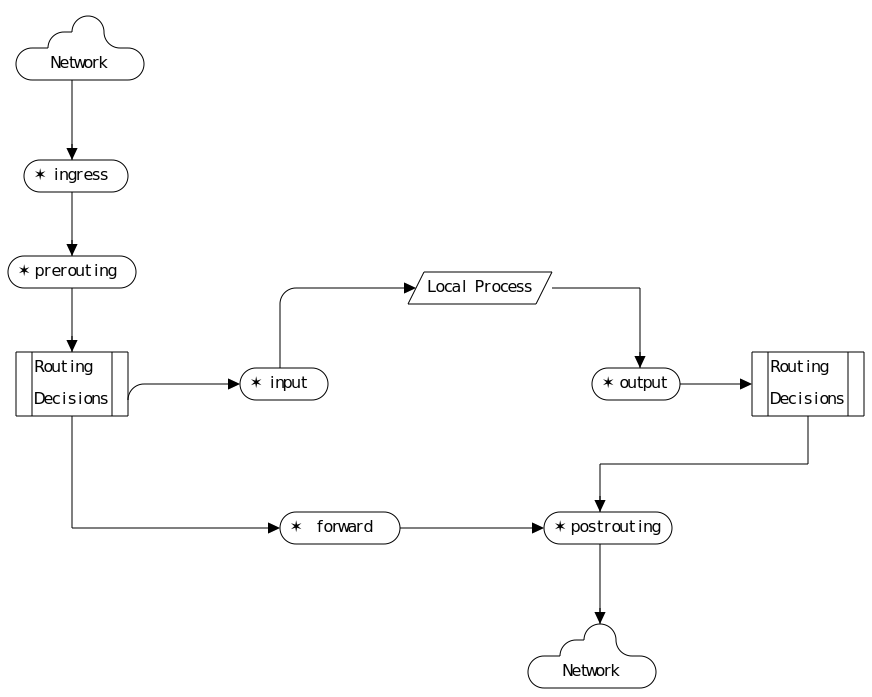
\includegraphics[width=\linewidth]{flow.eps}
    \caption{Schema del flusso di pacchetti in ftables}
    \label{fig:flow}
\end{figure}
Lo schema rappresenta i possibili percorsi di un pacchetto: l'asterisco
evidenzia gli hook ai quali si possono associare le catene contenenti le
regole:
\begin{itemize}
    \item ingress
    \item prerouting
    \item input
    \item output
    \item forwarding
    \item output
    \item postrouting
\end{itemize}
La possibilit\`a di intervenire precocemente sul pacchetto, appena il driver
dell scheda di rete lo passa al livello superiore, \`e utile per gestire
attacchi tipo DDoS o per limitare la banda senza appesantire il lavoro del
kernel: questo \`e reso possibile dall'hook ingress che interviene prima del
prerouting. Catene associate all'hook ingress sono definite in tavole della
famiglia netdev. Scartare i pacchetti a questo livello \`e due volte
pi\`u efficiente rispetto al drop in prerouting.

I pacchetti che sono destinati a qualche processo locale (cioè sono indirizzati
all'host stesso) sono gestiti tramite l'hook input ed analogamente quelli
generati da processi locali tramite l'hook output.

Il traffico che deve essere inoltrato fra le due reti viene gestito tramite
l'hook forward. Il NAT interviene in prerouting (DNAT) e postrouting (SNAT).

Il layout iniziale di nftables \`e semplicemente l'insieme vuoto,
l'amministratore \`e libero di configurare tavole (table) e catene
(chain)\footnote{Le tavole sono contenitori di catene che a loro volta
contengono regole.} nel modo ritenuto pi\`u adatto al problema da risolvere.

Nemmeno i contatori sono attivi per default, a differenza di iptables:
devono essere esplicitamente attivati quando necessario, migliorando
cos\`i le prestazioni. Il fatto di poter indicare pi\`u azioni per una regola
rende maggiormente leggibile e consistente il codice;
con iptables spesso è necessario saltare ad un'altra catena contenente le diverse
azioni. Ad esempio, log e drop con iptables:

\begin{lstlisting}
# iptables -t filter -A OUTPUT -d 10.0.0.1 -j LOG # Log, continue to next rule
# iptables -t filter -A OUTPUT -d 10.0.0.1 -j DROP # Drops the same packet
\end{lstlisting}
oppure 
\begin{lstlisting}
# iptables -t filter -N LOGGING # Create non-base chain for logging
# iptables -t filter -A LOGGING -j LOG # Add rule to logging chain to LOG
# iptables -t filter -A LOGGING -j DROP # Add rule to logging chain to DROP
# iptables -t filter -A OUTPUT -d 10.0.0.1 -j LOGGING # Jump LOGGING if match
\end{lstlisting}
con nftables \`e sufficiente una sola regola:
\begin{lstlisting}
# nft add rule ip filter output ip daddr 10.0.0.1 log drop
\end{lstlisting}
Un esempio minimale di configurazione per un server web pu\`o essere
il seguente:
\lstinputlisting[caption=Semplice esempio per server web, style=customc]{nftables-web.conf}
Notare, riga 9, che le connessioni già stabilite o relative a
connessioni già stabilite, informazione ricavata dalla conntrack table,
sono accettate.
I servizi raggiungibili dall'esterno sono ssh, http e https, tutto il resto
viene ignorato (drop) senza inviare "ICMP host unreachable". Inoltre i
pacchetti rifiutati vengono contati (counter).

\lstinputlisting[caption=Semplice esempio di router/firewall, style=customc]{nft-simple-forward.nft}
Questo esempio descrive il comportamento di un semplice
router/firewall. La tavola è associata ai protocolli IPv4 e IPv6 (inet) e
definisce due insiemi contenenti indirizzi dei due tipi (righe 2 e 7).
Al solito viene accettato traffico relativo a connessioni attive (riga 13)
mentre viene ignorato traffico non valido (causato da stealth port scan, da
problemi nella conntrack table o da anomalie benigne).
Oltre ad accettare connessioni verso qualsiasi server ssh e http(s), un
verdetto positivo è previsto anche per qualsiasi connessione verso i server
elencati ei due insiemi my\_ipv4\_addrs e my\_ipv6\_addrs.
Per ognuna delle categorie sopra elencate viene attivato il contatore.

\section{Strumenti di debug e tracing}
Ritengo che il sistema di tracing offerto da nftables sia di ottima qualit\`a;
\`e fondamentale per la rapida individuazione dei bug durante la
sperimentazione e lo sviluppo dei ruleset.
Il tracing viene attivato impostando una metainformazione relativa al pacchetto: nftrace=1.
\begin{lstlisting}
# nft add rule filter forward udp dport 53 meta nftrace set 1
\end{lstlisting}
Dal momento che transita dalla catena di forward, ogni pacchetto destinato ad un DNS server riporter\`a
i dettagli del suo percorso attraverso l'insieme di regole.
Per osservare il resoconto del viaggio del pacchetto \`e necessario attivare il
monitor da console: i pacchetti con nftrace settato invieranno al monitor le informazioni
con tutti i dettagli relativi al percorso seguito.
Questo ad esempio \`e il percorso di un pacchetto destinato ad un DNS server:
\begin{lstlisting}[style=customc]
# nft monitor
trace id e7d627c0 ip captive forward packet: iif "eth1" oif "eth0" 
      ether saddr 00:16:3e:05:12:55 ether daddr 00:16:3e:35:e7:80 
      ip saddr 193.168.100.159 ip daddr 8.8.8.8 
      ip dscp cs0 ip ecn not-ect ip ttl 63 ip id 36018 ip length 59 udp sport 40220 
      udp dport domain udp length 39 @th,64,96 49749720051147984142130479104
trace id e7d627c0 ip captive forward rule udp dport domain nftrace 
      set 1 (verdict continue)
trace id e7d627c0 ip captive forward verdict continue
trace id e7d627c0 ip captive forward
trace id e7d627c0 ip captive nat_postrouting verdict continue
trace id e7d627c0 ip captive nat_postrouting
\end{lstlisting}

\chapter{Migrazione del Captive Portal}

%Il progetto che sto realizzando prevede molte attivit\`a, ad esempio gli
%automatismi di gestione delle regole tramite l'uso di git e Ansible.

Per Captive Portal si intende una configurazione della rete in cui il
dispositivo che si collega la prima volta viene reindirizzato ad una pagina web
tramite la quale si identifica ottenendo l'autorizzazione all'uso della rete.

Nel nostro caso l'identificazione avviene fornendo il numero di cellulare al
quale viene inviato un codice via SMS. L'utente restituisce questo codice
attraverso la stessa pagina del Captive Portal e cos\`i facendo il dispositivo
viene autorizzato: il mac address viene aggiunto dinamicamente tra quelli
che il firewall non deve bloccare.

Lo schema di verifica e autorizzazione del traffico è il seguente:
\begin{enumerate}
    \item il pacchetto viene analizzato per verificare se il mac
    address è stato autorizzato
    \begin{itemize}
        \item sì: allora finisce l'analisi e il pacchetto viene inoltrato
        \item no: il pacchetto viene marcato (0x63)
    \end{itemize}
    \item in fase di prerouting, se il pacchetto è marcato ed la porta di
    destinazione è http allora viene reindirzzato (DNAT) alla pagina del
    captive portal
    \item negli altri casi (pacchetto marcato e traffico non http) allora il
    pacchetto viene scartato in fase di forwarding
\end{enumerate}

\section{Captive Portal con iptables}
\label{lab:captive}
La configurazione di iptables che realizza quanto descritto sopra è la
seguente:
\lstinputlisting[caption=Mangle per wifi free, style=customc,
label={lst:iptables-wifi}]{captive-iptables.conf}
Il listato \ref{lst:iptables-wifi} rappresenta la configurazione del
firewall limitatamente alle regole strettamente necessarie a realizzare la
funzionalità di captive portal. Il fatto di aver eliminato le regole non
pertinenti il caso in esame può far sembrare inutili o ridondanti alcune di
quelle elencate.

Le prime nove righe sono relative alla marcatura in fase di prerouting:
\begin{itemize}[itemindent=2em]
    \item[(riga 4)] il traffico proveniente dalla rete wifi (192.168.16.0/20)
    verrà analizzato dalla catena internet (salta alla riga 8)
    \item[(riga 8)] se il mac address sorgente è contenuto nel set captive\_ok
    ritorna
    \item[(riga 9)] marca il pacchetto con il valore 0x63 (99 decimale)
  \end{itemize}
  La tavola filter, riga 11:
  \begin{itemize}[itemindent=2em]
    \item[(riga 12)] di default scarta i pacchetti che non soddisfano una delle regole
    \item[(riga 13)] accetta il traffico relativo a connessioni già attivo
    \item[(riga 14)] scarta i pacchetti marcati con il valore 0x63
\end{itemize}
La tavola di NAT ha il compito di indirizzare il traffico http verso il sito
del captive portal.
Le righe dalla $20$ in poi sono relative all'insieme che contiene i mac
address autorizzati\footnote{Gli indirizzi non sono quelli reali perché anche
il mac address è un dato personale e agli utenti non è stato notificato un uso
di questo tipo dei loro dati.}, captive\_ok:
l'intestazione descrive la struttura dati di tipo hash di mac address e a
seguire sono elencati gli elementi dell'insieme.

\section{Captive Portal nella versione nftables}
Il porting ad nftables della logica sopra descritta è il seguente:
\lstinputlisting[caption=Captive portal con nftables, style=customc,
label={lst:nftables-wifi}]{captive-nftables.conf}
Possiamo intanto notare due cose:
\begin{itemize}
	\item il linguaggio prevede la definizione di variabili
	
	\item le due chain filter\_prerouting e nat\_prerouting sono di tipo diverso
	(cioè eseguono azioni diverse) ma sono agganciate allo stesso hook (prerouting),
	la priorità definisce quale deve essere l'ordine di consultazione
\end{itemize}
L'attivazione di un dispositivo si effettua inserendone il mac address nell'insieme
captive\_ok\footnote{In questo caso usiamo la sintassi da linea di comando invece che quella strutturata da script.}:
\begin{lstlisting}
# nft add element captive captive_ok {00:16:3e:05:12:55}
\end{lstlisting}

\section{Autorizzazioni temporizzate}

Possiamo ora sfruttare funzionalità spcifiche di nftables.  Vogliamo che
l'autorizzazione all'uso della rete wifi scada dopo 15 giorni.  Per fare ciò
dobbiamo modificare la definizione del set, alla riga 5 del listato
\ref{lst:nftables-wifi}, introducendo un timeout\footnote{Al momento \`e aperto
un bug report perch\'e non si riescono ad impostare timeout > 24d20h31m23s:
\url{https://bugzilla.netfilter.org/show\_bug.cgi?id=1237}} in questo modo:
\begin{lstlisting}[style=customc, firstnumber=5]
set captive_ok { type ether_addr; timeout 15d; }
\end{lstlisting}
Ora ogni elemento inserito nell'insieme verrà automaticamente eliminato dopo 15
giorni e sarà possibile verificare in ogni momento quanto tempo resta prima
della scadenza:
\begin{lstlisting}[style=customc]
# nft add set captive captive_ok_timeout { type ether_addr\; timeout 15d\; }
# nft list set captive captive_ok_timeout
table ip captive {
        set captive_ok_timeout {
                type ether_addr
                timeout 15d
        }
}
# nft add element captive captive_ok_timeout {6c:0b:84:91:7d:a4}
# sleep 5 && nft list set captive captive_ok_timeoulat
table ip captive {
        set captive_ok_timeout {
                type ether_addr
                timeout 15d
                elements = { 6c:0b:84:91:7d:a4 expires 14d23h59m54s }
        }
}
\end{lstlisting}
Ovviamente un elemento inserito successivamente avrà il proprio timer:
\begin{lstlisting}[style=customc]
# nft add element captive captive_ok_timeout {02:0a:76:09:41:8b}
# nft list set captive captive_ok_timeout
table ip captive {
        set captive_ok_timeout {
                type ether_addr
                timeout 15d
                elements = { 02:0a:76:09:41:8b expires 14d23h59m57s,
                             6c:0b:84:91:7d:a4 expires 14d23h56m4s }
        }
}
\end{lstlisting}
Alternativamente o in aggiunta al timeout di default, è possibile definire un
set in cui ogni elemento può essere esplicitamente dichiarato con il proprio
timeout:

\begin{lstlisting}
# nft add set captive captive_ok_timeout_flag { type ether_addr\; flags timeout\; timeout 15d\; }
# nft add element captive captive_ok_timeout_flag {02:0a:76:09:41:8b}
# nft list set captive captive_ok_timeout_flag
table ip captive {
        set captive_ok_timeout_flag {
                type ether_addr
                timeout 15d
                elements = { 02:0a:76:09:41:8b expires 14d23h59m57s }
        }
}
# nft add element captive captive_ok_timeout_flag {02:0a:88:01:c3:51 timeout 42m}
# nft list set captive captive_ok_timeout_flag
table ip captive {
        set captive_ok_timeout_flag {
                type ether_addr
                timeout 15d
                elements = { 02:0a:76:09:41:8b expires 14d23h58m51s,
                             02:0a:88:01:c3:51 timeout 42m expires 41m58s }
        }
}
\end{lstlisting}
Questa caratteristica dei set alleggerisce il lavoro di gestione del sistema, in quanto non è necessario intervenire con altri
strumenti per eliminare i mac address scaduti.
\section{Aggiornamento del timeout}
In realt\`a sarebbe auspicabile un comportamento pi\`u {\em intelligente}: se un utente \`e 
un ospite frequente\footnote{Ad esempio perch\'e dipendente.} vorremmo evitare
di chiedergli la registrazione ogni 15 giorni,
vogliamo invece far scadere l'autorizzazione 15 giorni dopo l'ultimo utilizzo del servizio.
Per ottenere ci\`o \`e necessario aggiornare il timeout
ogni volta che si osserva transitare un pacchetto generato dal singolo client.

Nftables consente di agire sui set aggiornandoli dinamicamente in funzione del
percorso del pacchetto ed \`e proprio questa la funzionalit\`a che ci serve.
Riscriviamo quindi le regole dello script \ref{lst:nftables-wifi} cos\`i:

\begin{lstlisting}[style=customc,firstnumber=5]
...
chain filter_prerouting {
    type filter hook prerouting priority 0; policy accept;
    ip saddr $WIFINET ether saddr @captive_ok set update ether saddr timeout 15d @captive_ok return
    ip saddr $WIFINET mark set 0x63
}
...
\end{lstlisting}
La riga numero 8 del listato \ref{lst:nftables-wifi} adesso, non solo ritorna,
di fatto autorizzando il pacchetto, ma contestualmente aggiorna l'elemento
nell'insieme, reimpostandone la validit\`a a 15 giorni.

Questa funzionalit\`a realizzata a livello applicativo avrebbe significato
doversi confrontare con almeno tre domini diversi: le regole del firewall, il
database delle autorizzazioni e i log. La soluzione sarebbe sicuramente di non
facile realizzazione, soggetta a difetti e comunque difficile da monitorere e
debuggare.

\section{Limitazione della banda}

Potrebbe essere utile imporre dei limiti di banda utilizzata da parte degli
utenti della rete wifi. Anche in questo caso nftables offre una soluzione che
risulta anche semplice da implementare in quanto anche in questo caso si
integra in modo naturale nel linguaggio di definizione delle regole.

Il caso pi\`u semplice consiste nel limitare la banda occupata globalmente
dalla rete wifi (facciamo sempre riferimento allo script \ref{lst:nftables-wifi}):

\begin{lstlisting}[style=customc,firstnumber=18]
chain forward {
    type filter hook forward priority 0; policy accept;
    limit rate over 8 mbytes/second drop
    ct state established,related accept
    mark 0x63 drop
}
\end{lstlisting}
Avendo introdotto la riga 20 imponiamo che il traffico inoltrato non possa
superare 8 mbytes, i pacchetti in eccesso vengono scartati.

Questa limitazione di banda risulta pi\`u efficiente\footnote{Vedi ad esempio
\url{https://netdevconf.org/1.2/slides/oct6/08\_nftables\_Load\_Balancing\_with\_nftables\_II\_Slides.pdf}}
se configurata sfruttando l'hook ingress disponibile nella famiglia netdev.
Nella configurazione delle regole per il Captive Portal ho scelto questo
approccio.
\begin{lstlisting}[style=customc,firstnumber=18]
table netdev wifirate {
    chain download {
        # interfaccia verso
        type filter hook ingress device eth2 priority 0;
        limit rate over 8 mbytes/second counter drop
    }
    chain upload {
        # interfaccia verso wifi
        type filter hook ingress device eth1 priority 0;
        limit rate over 8 mbytes/second counter drop
    }
}
\end{lstlisting}
La tabella wifirate limita la banda entrante dall'interfaccia eth2, download da internet,
e quella entrante da eth1 cio\`e l'upload verso internet.

Una configurazione leggermente pi\`u articolata potrebbe dover distinguere e
trattare differentemente diverse tipologie di traffico. Ad esempio potremmo
decidere di limitare la banda per il download ma solo per la rete wifi:
\begin{lstlisting}[style=customc,firstnumber=20]
ip daddr $WIFINET limit rate over 6 mbytes/second burst 10 mbytes/second drop
\end{lstlisting}
L'opzione di burst consente di usufruire di maggiore banda temporaneamente.

Una regola ancora pi\`u raffinata potrebbe essere la seguente dove sfruttiamo
i meter e la funzione di concatenazione realizzata dalĺ'operatore ".":
\begin{lstlisting}[style=customc,firstnumber=20]
ip daddr $WIFINET meter rate-meter { ip saddr . ip daddr limit rate over 3 mbytes/second burst 5 mbytes/second } drop
\end{lstlisting}
In questo caso le limitazioni sono per coppie di indirizzi sorgente e destinazione,
il punto concatena i due indirizzi generando la chiave dell'elemento nel meter.

\chapter{Strumenti di sviluppo e test}

Per poter agire in sicurezza e pi\`u celermente ho preferito lavorare in un
ambiente completamente virtualizzato.

\section{Virtualizzazione}
Per realizzare i test delle regole in un ambiente simulato, ho configurato tre
server virtuali libvirt+lxc, cio\`e sostanzialmente tre Linux container.  Il
sistema operativo sia dell'host che dei tre guest \`e Debian 9.4 (stretch) e
l'hardware consiste di un laptop Intel i5 dual core.

Una delle tre macchine, chiamata fw, simula il firewall tra una LAN e una rete
pubblica, la seconda, chiamata pc, rappresenta una macchina all'interno della rete
locale mentre la terza simula un server in internet, chiamato wikipedia.

Lo strato di virtualizzazione della rete \`e quello offerto da libvirt e
definisce le reti loc e net rispettivamente per la LAN e per internet.
\begin{figure}[H]
\begin{center}
      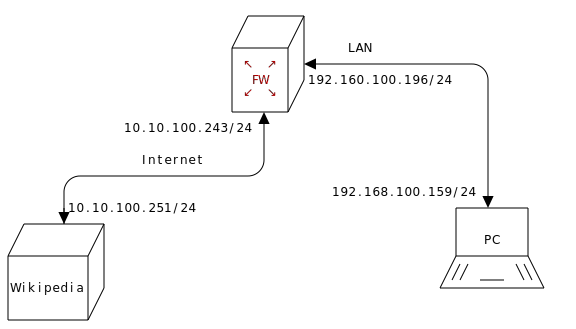
\includegraphics[width=.7\linewidth]{vnet.eps}
      \caption{Macchine virtuali}
      \label{fig:vnet}
\end{center}
\end{figure}
In questa configurazione le prestazioni della rete sono state valutate con iperf(1).
\begin{center}
  \label{tab:benchmark}
  \begin{table}[ht]
    \centering % used for centering table
     \begin{tabular}{@{}llcc@{}}
     \toprule
     {\bf Configurazione} & {\bf iperf} & {\bf wget 4GB} \\ \midrule
         routing  & 32.6                & 4.5 \\
         mark     & 30.3                & 4.4 \\ 
         mark-full& 30.2                & 4.4 \\ \bottomrule
      \end{tabular}  
    \caption{Benchmark} % title of Table
  \end{table}
\end{center}
\section{Debug}

Il debug come accennato in precedenza \`e stato facilitato dal sistema di
packet tracing.

Ovviamente fondamentali i tool tradizionali, uno su tutti tcpdump.

Volendo scendere ad un pi\`u basso livello si pu\`o arrivare a
verificare il byte code, iniettato nel kerneli quando si inserisce una regola:
\begin{lstlisting}[style=customc]
# nft --debug=netlink add rule atable arule ip saddr 10.0.0.0/8 accept            
ip atable arule
  [ payload load 4b @ network header + 12 => reg 1 ]
  [ bitwise reg 1 = (reg=1 & 0x000000ff ) ^ 0x00000000 ]
  [ cmp eq reg 1 0x0000000a ]
  [ immediate reg 0 accept ]
\end{lstlisting}
Il payload \`e il pacchetto in esame. Alla riga 3 vengono caricati, nel
registro numero 1, 4 byte a partire dalla dodicesima posizione dell'header del
pacchetto: cio\`e l'indirizzo IPv4 sorgente. Alla riga 4 viene applicata la
netmask per estrarre il byte pi\`u significativo che alla riga 5 viene
confrontato con 0xa (10 decimale): se il confronto ha successo il pacchetto
viene accettato.

\chapter{Considerazioni finali}

Nonostante gli indiscutibili vantaggi di nftables rispetto ad iptables, non
sembra che la sostituzione possa avvenire a breve.  La difficolt\`a di nftables
nello scalzare iptables dipende dal fatto che iptables nei sui 17/18 anni di
vita si \`e diffuso molto (datacenter, virtualizzazione, container, \ldots) ed
ha accresciuto le funzionalit\`a, magari in modo non elegante ma comunque
efficace. Per certi versi la situazione assomiglia a quella di ``IPv4 vs
IPv6''.

Paradigmatica a questo proposito \`e la decisione presa da WikiMedia Foundation
dopo aver discusso sull'argomento {\em netfilter software at WMF: iptables vs
nftables}, vedi  \url{"https://phabricator.wikimedia.org/T187994"}.  La
proposta di migrare l'infrastruttura di WMF \`e stata avanzata da Arturo
Borrero, mantainer del pacchetto nftables per Debian e operator del cloud team
di Wikimedia, e lui stesso conclude che non \`e il momento:
\begin{quote}
    EOF. I propose we follow up in the future.
\end{quote}
Borrero stesso aveva comunque previsto fino a 2
anni di lavoro per la migrazione completa ad nftables dell'intera
infrastruttura.

Come nel caso di WikiMedia per molti il ragionamento sembra essere lo stesso: ``tutto sta
funzionando con iptables, non si evidenziano problemi, lo sforzo per passare a
nftables \`e importante: non conviene.''.

\section{eBPF}

Quello che invece sembra rappresentare il futuro del Linux Firewall \`e eBPF,
enanched Berkeley Packet Filtering\footnote{eBPF fa molto di pi\`u che filtrare
pacchetti: \`e anche in grado di fare raw tracing in modo simile a quello di
DTrace e SystemTap. Un buon punto di partenza \`e
\url{https://github.com/iovisor/bcc}}.
L'articolo su Linux Weekly News del 19 febbraio 2018
\footnote{\url{https://lwn.net/Articles/747551/}} dal titolo ``BPF comes to firewalls''
dice tra l'altro:

\begin{quote}
\ldots Miller\footnote{Si tratta di David Miller, uno dei mantainer dello stack
TCPI/IP di Linux} said in the discussion that nftables failed to address the
performance problems in Linux's packet-filtering implementation, driving users
toward user-space networking technologies instead. There is a real possibility
that nftables could end up being one of those experiments that is able to shed
some light on the problem space but never takes over in the real world.
\end{quote}


\section{eBPF/XDP}
Quando abbiamo visto i possibili utilizzi dell'hook ingress consideravamo
un vantaggio in termini di prestazioni quello di essere ``pi\`u vicini'' al
driver della scheda di rete. XDP (eXpress Data Path) si spinge oltre
demandando il filtraggio, e altro, direttamente al firmware della scheda di
rete (vedi \url{https://www.iovisor.org/technology/xdp}).

Ci sono gi\`a produttori di SmartNIC\footnote{Ad esempio
    \url{https://www.netronome.com/products/smartnic/overview/}}, cio\`e di
    schede di rete progettate apposta per affrancare il server 
    da compiti sempre pi\`u complessi (offloading).  Qualcuno
    non vede di buon occhio questo approccio perch\'e teme si possa trattare di tentativi di
    ``kernel
    bypass'' ma gli sviluppatori di soluzioni eBPF/XDP assicurano che ci\`o
    non si
    verificher\`a\footnote{\url{https://www.netronome.com/blog/avoid-kernel-bypass-in-your-network-infrastructure/}}.

\section{Conclusioni}

Visto il fermento intorno alle nuove soluzioni di packet filtering,
considerando il fatto che iptables funziona ed \`e tuttora il framework
indiscusso per quanto riguarda il packet filtering e non c'\`e dubbio che non
verr\`a abbandonato nell'immediato futuro, le ricadute pratiche del lavoro di
sperimentazione svolto si limiteranno alla messa in produzione di nftables
limitatamente al Captive Portal in virt\`u delle funzionalit\`a di cui abbiamo
discusso nella sezione \ref{lab:captive}.


%----------------------------------------------------------------------------------------
%	THESIS CONTENT - APPENDICES
%----------------------------------------------------------------------------------------

\appendix % Cue to tell LaTeX that the following "chapters" are Appendices

% Include the appendices of the thesis as separate files from the Appendices folder
% Uncomment the lines as you write the Appendices

%\include{Appendices/AppendixA}
%\include{Appendices/AppendixB}
%\include{Appendices/AppendixC}

%----------------------------------------------------------------------------------------
%	BIBLIOGRAPHY
%----------------------------------------------------------------------------------------

\printbibliography[heading=bibintoc]

%----------------------------------------------------------------------------------------

\end{document}  
